\lab{Nearest Neighbor Search}{Nearest Neighbor Search}
\label{lab:NNS}

\objective{Introduce the nearest neighbor search problem, K-D trees, and the curse of dimensionality.}%Teach about branch and bound and the curse of dimensionality using the nearest neighbor search problem.}

\section*{The Nearest Neighbor Search Problem}

The nearest neighbor search problem is an optimization problem that arises in many applications, including computer vision, pattern recognition, internet marketing, and data compression.
The premise is this: suppose that you move into a new city with several post offices.
Since you are a busy individual, to minimize travel time you would like to know which post office is closest to your home.
More generally, the problem is to find the point in a set of points (the post offices) that is nearest to some other point (your home).

% Problem 1: Euclidean Distance
\begin{problem}
To solve the nearest neighbor problem, we must define a metric.
That is, we need a way of determining the distance between two points.
For this lab, we will use standard euclidean distance.

% should we say 1 x n (like usual) or 1 x k (to reflect the k-d tree idea)
Write a function that accepts two vectors (as $1$ x $k$ numpy arrays) and returns the distance between them.
If the two vectors do not have the same dimensions, raise a ValueError.
Make sure the function can handle data in $\mathbb{R}^n$ for any $n\in\mathbb{N}$
\end{problem}


The naive approach to solving the post office problem is to travel from your house to one of the post offices, then from your house to a different post office, and so on until all post offices have been visited. Then choose the post office that it took the least amount of time to get to from your house. This exhaustive method is clearly inefficient, and only feasible if the data set is very small.

% Problem 2: Exhaustive search method
\begin{problem}
Write a function that solves the nearest neighbor search problem by exhaustively checking all of the distances between a point of interest and each point in a data set.

% what should the format of the data be?
The function should take in the set of data points (as a $m$ x $k$ numpy array) and a single target point (as a $1$ x $k$ numpy array).
Return the point in the set that is closest to the point of interest (the nearest neighbor) and the distance between those two points. As in the previous problem, your function should be able to take in data in $\mathbb{R}^n$ for any $n\in\mathbb{N}$.
\end{problem}

% Bad choice of variables k and n
The complexity of this algorithm is $O(kn)$, where $k$ is the number of dimensions and $n$ is the number of data points.

\section*{K-D Trees}

\begin{figure}
\caption{This 2-dimensional tree partitions $\mathbb{R}^2$ at each level. (TODO: Make a figure like the one on Wikipedia or reference Wikipedia)}
\label{fig:k-binary-search}
\end{figure}

Fortunately, there is a particular data structure that lends itself well to solving this problem quickly.
A \emph{k-d tree}, or \emph{k-dimensional tree}, is a specialized binary search tree.
Using a k-d tree to solve a nearest neighbor search problem speeds things up by travelling toward the target incrementally instead of exhaustively searching every option.
Just as a regular binary search tree partitions the number line at every step of descent, a k-d tree partitions $\mathbb{R}^k$ at every step of descent.

At each level of the tree, for some $i$ the nodes to the left of the parent nodes have a lower value in the $i^{th}$ dimension and the nodes to the right of the parent node have a greater value in the $i^{th}$ dimension.
The choice of dimension $i$ cycles through the possible choices as we descend deeper through the tree.
In the $3$-dimensional case the root node is divided in the $x$ dimension, the children in the $y$ dimension, the grandchildren in the $z$ dimension, the great-grandchildren in the $x$ dimension, and so on.
See figure \ref{fig:k-binary-search} for an example in $\mathbb{R}^2$.

Constructing an optimal k-d tree requires sorting the data before each insertion, so the complexity is $O(n\log^2{n})$. However, once the tree is built we can use it as needed with much lower Big-O rates.

In this lab we will construct our own k-d tree class by inheriting from the previous lab's \li{BST} class. First, we need to create specialized nodes.

% KDT Node class -- should probably become example code instead of a problem
\begin{problem}
Copy or import your \li{BSTNode} class from the previous lab.
Write a \li{KDTNode} class that inherits from \li{BSTNode}.
% Optional vvv
Modify the constructor so that a \li{KDTNode} can only hold a list or numpy list.
% Optional ^^^
Add an attribute called \li{axis}.
This attribute will track how deep the node is in the tree so we know which entry of \li{data} to use as the bisector.

Write the \li{__lt__} and \li{__gt__} magic methods so that the $<$ and $>$ operators compare the $i^{th}$ entry of the data, where $i$ is the \li{axis} attribute of the node on the \emph{right side} of the operator.
For example,

\begin{lstlisting}
>>> x = KDTNode([1,2])
>>> y = KDTNode([3,1])
>>> y.axis = 0			# Compare the '0th' entry of the data 
>>> x < y				# True, since 1 < 3
True
>>> x > y
False

>>> y.axis = 1			# Compare the '1st' entry of the data
>>> x < y				# False, since 2 > 1
False
>>> x > y
True
\end{lstlisting}

Finally, write the \li{__sub__} magic method so that \li{x} - \li{y} yields the euclidean distance between the data in node \li{x} and the data in node \li{y}.

(Hint: use the function from problem 1)
\end{problem}


Now we must construct the actual k-d tree class.
The structure requires an attribute that houses the dimension of the tree (the \emph{k} of the k-d tree).

\begin{lstlisting}
def class KDT(BST)
	"""A k-dimensional tree object."""

	def __init__(self, k)
	"""Set the dimension attribute 'k'."""
		BST.__init__(self)
		self.k = k
\end{lstlisting}


The only major difference between a k-d tree and a binary search tree is how the data is compared at each depth level.
As long as we set the \li{axis} attribute correctly in each node as it is inserted into the tree, we should be able to do this fairly easily because of our work in the previous problem.
Though we don't need to use a \li{find} function in solving the nearest neighbor problem, we provide the k-d tree version of \li{find} as an instructive example.

\begin{lstlisting}
class KDT(BST):
	# ...

	def find(self, data):
		"""Return the node containing 'data'. Raise a ValueError if there is
		no such node in the tree or if the tree is empty."""
		
		def _step(current, target):
			"""Recursively approach the target node."""
			
			if current is None:				# Base case: target not found.
				return current
			if current.data == target.data:	# Base case: target found!
				return current
			if target < current:			# Recursively search to the left
				return _step(current.left, target)
			else:							# Recursively search to the right
				return _step(current.right, target)
			
		if self.root is None:				# Check for empty tree
			raise ValueError(str(data) + " is not in the tree.")
		
		# Create a new node so that the KDTNode comparison operators can be used
		n = KDTNode(data)
		found = _step(self.root, n)
		if found is None:					# Report that the data was not found
			raise ValueError(str(data) + " is not in the tree.")
		return found						# Return the node containing 'data'
\end{lstlisting}

At every comparison in the \li{_step} function, the data of \li{target} and \li{current} are compared based on the \li{axis} attribute of \li{current}, since \li{current} is the right-hand operand.
% A little repetitive here
This way if each existing node in the tree has the correct \li{axis}, the correct comparisons will be made as we descend.

% This next bit should probably be part of the next problem.
\begin{comment}
To solve the nearest neighbor search problem, we only need to create the k-d tree once. Then we can use it multiple times with different target points. To prevent the user from messing with the tree, disable the \li{remove} method:
\begin{lstlisting}
class KDT(BST):
	# ...
	
	def remove(self, *args):
		raise ValueError("remove() has been disabled for this class.")
\end{lstlisting}
\end{comment}

\begin{problem}
Finish the \li{KDT} class by overriding \li{insert} and disabling \li{remove}.

To insert a new node, first check to make sure the data is the proper format. Then find the correct insertion location using an approach similar to the \li{find} method. Remember to double-link the nodes. Set the \li{axis} of the new node appropriately. Do not allow for duplicates in the tree.

To solve the nearest neighbor search problem, we need only create the k-d tree once. Then we can use it multiple times with different target points. To prevent the user from altering the tree, disable the \li{remove} method. Raise a \li{ValueError} if the method is called, and allow it to receive any number of arguments.

\end{problem}


Now that we have a k-d tree, we can use it to solve the nearest neighbor problem.
First we must load the tree with data so that it can be searched.

% This can be done by writing the following short function, or by adding stuff to the constructor of the KDT class.
% I like the constructor idea, but I have only written it so far as a function.
% This could also possibly be absorbed into the next problem.
\begin{problem}
Write a function that creates a \li{KDT} instance and loads it with a set of data.
The data will be a $m$ x $k$ numpy array.
For an optimal k-d tree, the data needs to be inserted in a very particular order.
However, inserting at random still usually produces a good tree.
For this problem, insert the data in the order that it is given (iterate through the rows).
\end{problem}

To solve the nearest neighbor problem, we need to do a careful recursive search through the tree.
At each step, we need to keep track of a current search node, the target point, the current best point (our current candidate for the nearest neighbor), and the current minimum distance (the distance from the nearest neighbor to the target).
We start the algorithm on the root node.
For each recursive step, we first check if the euclidean distance between the current search node and the target point is less than the current minimum distance.
If so, we update the nearest neighbor and calculate the new minimum distance.
We then descend through the tree and search recursively, similar to the \li{find} function.

We aren't done, however; after descending we need to check that there truly is no other nearest neighbor.
Technically, we are checking to see if the hypersphere of radius `minimum distance' around the supposed nearest neighbor does not intersect with any other hyperplanes created by the tree.
In the code we accomplish this by adding the minimum distance to the $i^{th}$ entry of the target point's data, where $i$ is the \li{axis} of the supposed nearest neighbor.
If this sum is greater than the $i^{th}$ entry of the current search node's data, then we need to descend in the \emph{opposite} direction that we came.

We summarize the algorithm below.

\begin{algorithm}
\begin{algorithmic}[1]
%d = euclidean\_metric
\Procedure{KDTSearch}{current, target, neighbor, distance}
\State index = current.axis
\State d = euclidean\_distance
	\If {d(current,target) $<$ distance}
		\State neighbor = current
		\State distance = d(current,target)
	\EndIf
	
	\If {target.data[index] $<$ current.data[index]}
		\State neighbor, distance = KDTSearch(current.left, target,
			\State									neighbor, distance)
		\If {target.data[index] + distance $>=$ current.data[index]}
			\State neighbor, distance = KDTSearch(current.right, target,
				\State									neighbor, distance)
		\EndIf
	\Else
		\State neighbor, distance = KDTSearch(current.right, target,
			\State									neighbor, distance)
		\If {target.data[index] + distance $<=$ current.data[index]}
			\State neighbor, distance = KDTSearch(current.left, target,
				\State									neighbor, distance)
		\EndIf
	\EndIf
\EndProcedure
\end{algorithmic}
\caption{k-d tree nearest neighbor search}
\label{alg:kdneighborz}
\end{algorithm}

\begin{comment}
\begin{algorithm}
\begin{algorithmic}[1]
\Procedure{KDSearch}{search\_point,parent\_node,b\_point,b\_distance,i}
    \If { Distance(search\_point,parent\_node.point) $<$ b\_distance }
        \State b\_point = parent\_node.point
        \State b\_distance = Distance from search\_point to parent\_node.point
    \EndIf

    \If{search\_point[i] $<$ parent\_node.point[i]}
        \State b\_point, b\_distance =
            \State KDSearch(search\_point,parent\_node.left\_child,b\_point,b\_distance,i+1)
        \If { search\_point[i] + b\_distance $geq$ parent\_node.point} 
            \State b\_point, b\_distance = 
                \State KDSearch(search\_point,parent\_node.right\_child,b\_point,b\_distance,i+1)
        \EndIf
    \Else
        \State b\_point, b\_distance = 
            \State KDSearch(search\_point,parent\_node.right\_child,b\_point,b\_distance,i+1)
        \If {search\_point[i] + b\_distance $leq$ parent\_node.point} 
            \State b\_point, b\_distance = 
                \State KDSearch(search\_point,parent\_node.left\_child,b\_point,b\_distance,i+1)
        \EndIf
    \EndIf
\EndProcedure
\end{algorithmic}
\caption{Nearest Neighbor}
\label{alg:nearestneighbor}
\end{algorithm}
\end{comment}


\begin{problem}
Use Algorithm \ref{alg:kdneighborz} to write a function that solves the nearest neighbor search problem by searching through a k-d tree.
The function should take in a k-d tree (already loaded with data) and a single point of interest.
Output the nearest neighbor in the tree and the distance from the nearest neighbor to the point of interest. 
\end{problem}

\section*{Scipy.spatial.KDTree}

Scipy has a built-in k-d tree structure.
It functions the same way that the \li{KDT} class does, except its operations have been heavily optimized.
To create the tree, we simply give it data in the initializer.
To solve the nearest neighbor search problem, we `query' the tree and give it a target point.
\li{query} returns a tuple of the minimum distance and the index of the nearest neighbor in the data.

\begin{lstlisting}
>>> from scipy.spatial import KDTree
>>> from numpy.random import random

# Initialize the tree with data
>>> data = random((100,20))
>>> scipy_kdt =  KDTree(data)

# Query the tree and print the minimum distance
>>> min_distance, node_index = scipy_kdt.query(random(20))
>>> print(min_distance)
1.1769198641683098

# Print the nearest neighbor by indexing into the tree's data
>>> print scipy_kdt.data[node_index]
array([ 0.30411204,  0.72439179,  0.81654881,  0.37483482,  0.37419281,
        0.19786408,  0.28339901,  0.26042625,  0.95736655,  0.9898518 ,
        0.3523297 ,  0.91607715,  0.91631037,  0.87982453,  0.66185015,
        0.8003657 ,  0.73600775,  0.7150884 ,  0.1836229 ,  0.89556912])
\end{lstlisting}

\section*{The Curse of Dimensionality}

In almost all multidimensional optimization problems, as the number of dimensions increases, the amount of time it takes to solve the problem increases exponentially.
This is the so-called `Curse of Dimensionality'.
In Algorithm \ref{alg:kdneighborz}, as the number of dimensions increases the number of times that we travel down both branches increases. Eventually using a k-d tree actually becomes less efficient than the exhaustive search method.

\begin{problem}
Write a function that creates three distinct figures.
In each figure, plot the time that it takes to solve the nearest neighbor search problem by exhaustive search, then by a k-d tree search using \li{KDT}, then again using \li{scipy.spatial.KDTree}.

In the first figure, use $n$ x 4 data sets with $n$ varying from 10,000 to 100,000 by multiples of 10,000.
Generate the data with \li{numpy.random.random()}.
Time only the searching of the k-d trees, not the building of them.

In the second figure, repeat the process with $n$ x 20 data sets, $n$ varying again from 10,000 to 100,000 by multiples of 10,000.

In the third figure, repeat the process with 20,000 x $k$ data sets, where $k$ varies from 2 to 50.
Here we are increasing the dimension, not the number of data points, and we expect to suffer from the curse of dimensionality.

\begin{figure}[H]
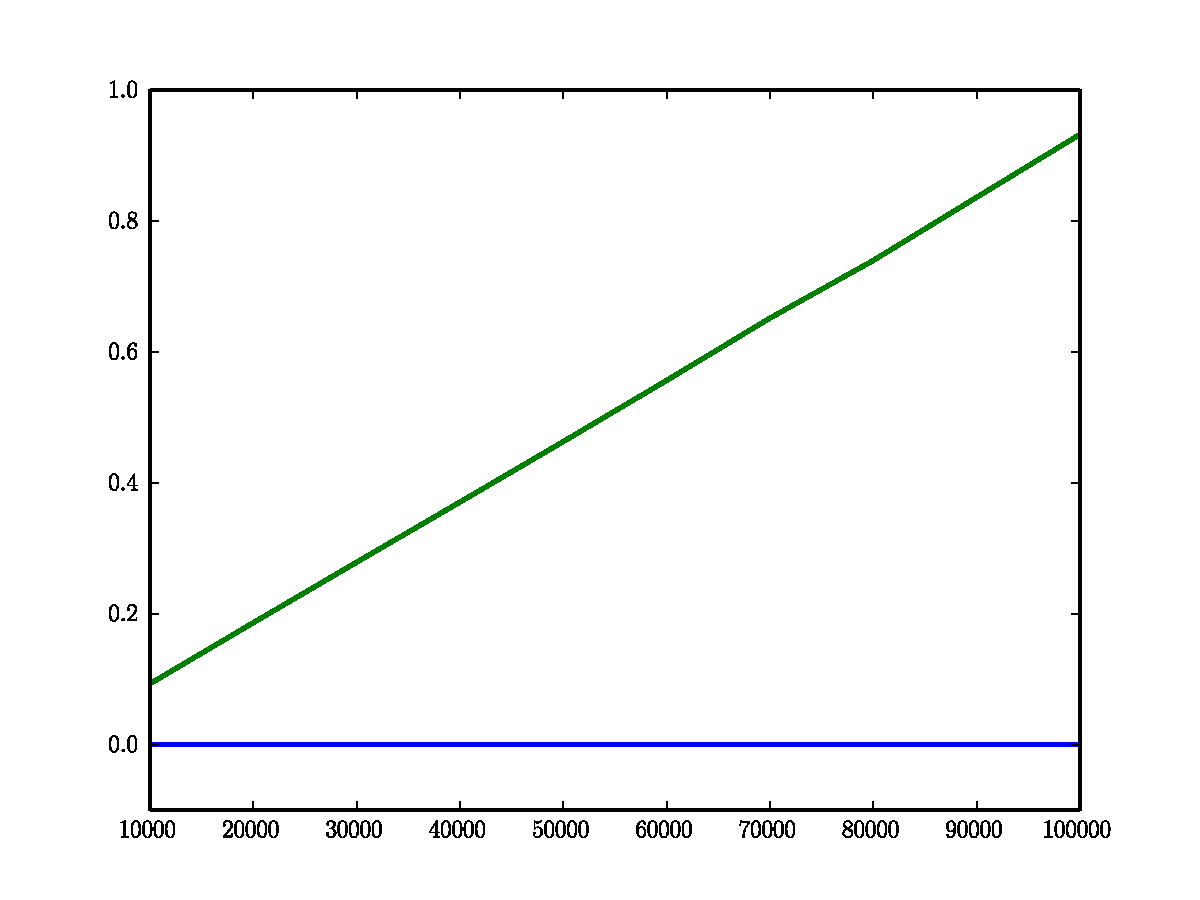
\includegraphics[width=\textwidth]{fourDTime.pdf}
\caption{The first plot may look something like this.
The green line is the naive algorithm and blue line is the kd-tree search.
The kd-tree is the clear winner so far.}
\label{fig:fourDTime}
\end{figure}

\begin{figure}[H]
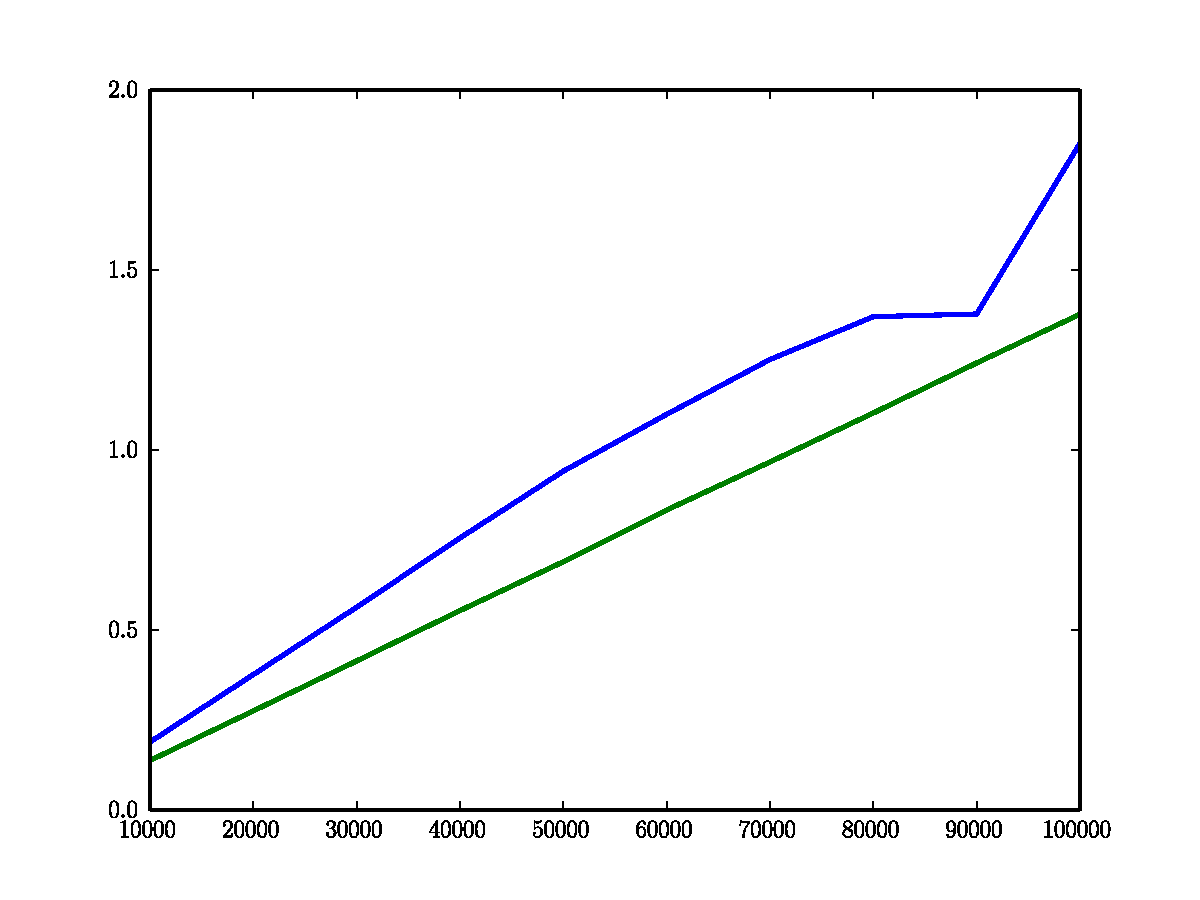
\includegraphics[width=\textwidth]{twentyDTime.pdf}
\caption{The second graph may look something like this.
The green line is the naive version and blue line is using a kd-tree.
Now the k-d tree search is slower than the naive algorithm.}
\label{fig:twentyDTime}
\end{figure}

\begin{figure}[H]
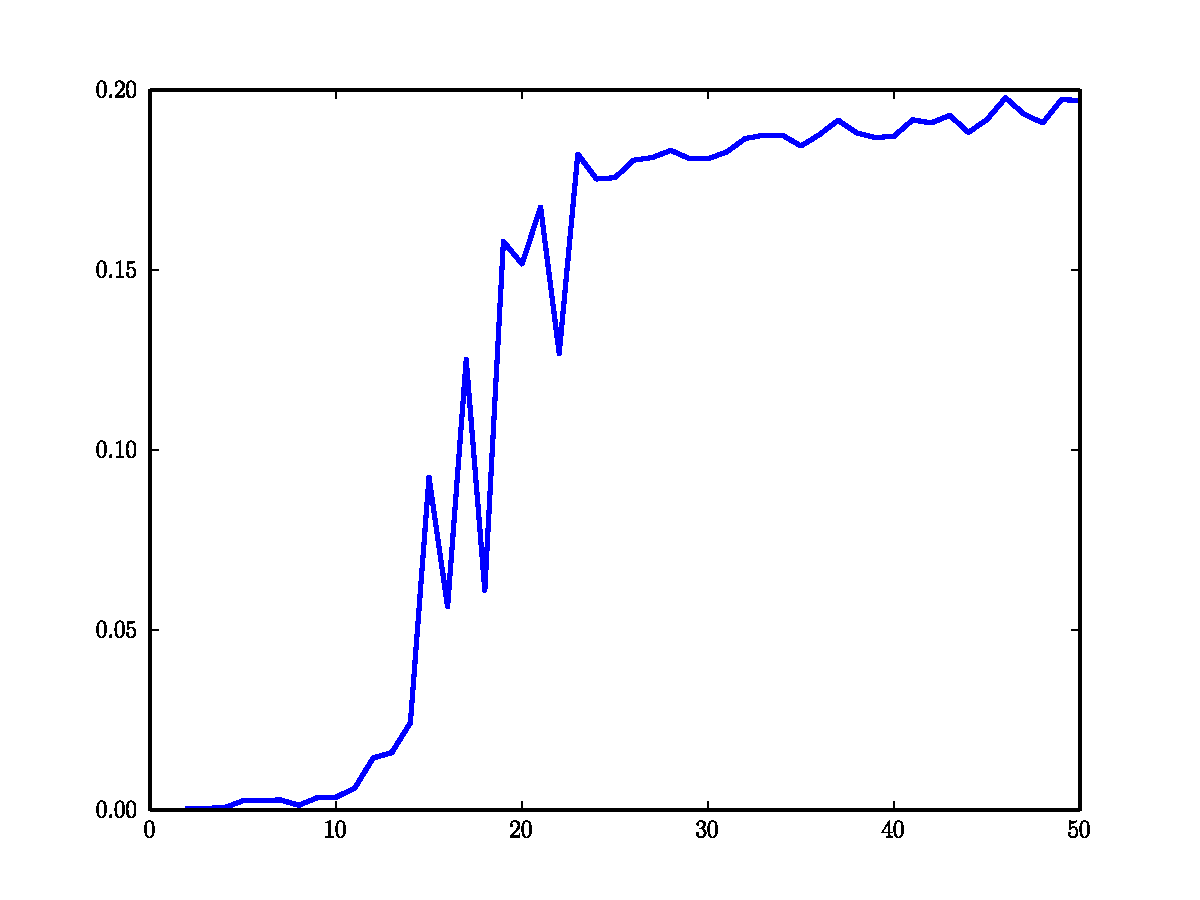
\includegraphics[width=\textwidth]{curseD.pdf}
\caption{The third graph may look something like this.
Around 15 dimensions the time spikes for the k-d tree search algorithm.
At that point using a kd-tree is even less effective than the naive algorithm.}
\end{figure}

\end{problem}

Certain algorithms suffer less due to the curse of dimensionality, but are not as good in lower dimensions.
Others, like the one we have studied in this lab, are good in lower dimensions but suffer heavily in higher dimensions.
Knowing how to pick your algorithm is an important skill in multidimensional data analysis.






\begin{comment} % END OF LAB. The rest of this needs to be moved elsewhere.

The complexity of this algorithm is $O(k\log(n))$ in optimal time.
Its worst case is $O(k*n^{1-\frac{1}{k}})$ where $k$ is the number of dimensions and $n$ is the number of points in the tree.
The reasons for this are discussed in the next section.

\section{Curse of Dimensionality}

As you increase the number of dimensions the number of times that you have to go down both branches increases.
You get to the point where you eliminate very few points by using a k-d tree.

\begin{problem}
Time both algorithms for the number of data points being $10,000-100,000$ every multiple of $10,000$ with $20$ dimensions.
Plot both times on the same plot. Now how do the two algorithms compare?
\end{problem}



\begin{problem}
Time the SciPy built in function for searching a k-d tree (do not time the building of the kd-tree) for the number of dimensions points being $2-50$ with $20,000$ data points.
Plot the time.
What do you notice?
\li{from scipy.spatial import KDTree} will import the built in k-d tree.
Create the tree by \li{tree = KDTree(data)} and search it by \li{tree.query(point)}.

\li{scipy.spatial} includes a \li{cKDTree} object which is implemented in C.
Is it any better?
\end{problem}


\section*{Classification}
A common problem is correctly classifying data.  
Suppose that you have a ten marbles, five of which are blue with a green stripe and the other five red with a purple stripe.  
If your friend gave you an eleventh marble that was blue with a brown stripe, which group would you put it in?  
Probably you would include it with the other blue marbles.  
What if the marble that your friend gave you was blue with a purple stripe?  
This marble shares characteristics with both groups.  
Where you end up grouping it will depend on which characteristics are most important to you.

This is the intuitive classfication problem.  
If we have data that is already grouped into distinct sets, into which set do we put new data?  
Classification has myriad and sundry applications.  
In this lab we will use it in the context of optical character recognition.

\section*{Nearest Neighbor Classification}
We will now more formally describe the classification problem and explain the nearest neighbor classification algorithm.  
Suppose we have a collection of vectors $\{x_1, ..., x_m\}$ in $\R^n$ with corresponding labels $\{l_1, ..., l_k\}$ describing to which group each datum belongs.  
This collection of vectors and labels is called our training set.  
Each entry of a vector is called a feature and $n$ is the size of our feature set.  
For example, consider the following vectors in $\R^3$

\begin{center}
\begin{tabular}{cc}
$(2,0,0)$ & $1$ \\
$(3,0,0)$ & $1$ \\
$(0,3,0)$ & $2$ \\
$(0,2,0)$ & $2$ \\
$(1/10,2,0)$ & $2$ \\
$(0,0,4)$ & $3$ \\
$(0,0,7)$ & $3$ \\
\end{tabular}
\end{center}

If we also have a metric on our space, we may determine the distance between all of these points.  
If we are given a new datum and we wish to decide which of the three groups to include it in, one option is to choose the group to which its closest neighbor belongs.  
Let us use the euclidean metric to classify $(0,0,5)$ against our training set.  
We see that the distance from $(0,0,5)$ and $(0,0,4)$ is only $1$, while the distance to the remaining points is at least $2$.  
The label of $(0,0,4)$ is $3$, and so we assign $(0,0,5)$ the same label.

Now, what if we wished to classify $(5/2,5/2,0)$?  
This presents a problem since this point is equidistant from the points in label $1$ and label $2$.  
In such a case it is up to the programmer to decide how to break the tie.

One case we need to consider is when the data that we are using in our search are on different scales. 
For example, suppose we wished to classify people applying for a loan at a bank as `risky' or `safe.'  
Further suppose that we know their age, education level, current debt, and how many credit cards they have.  
We could encode their education level as integers between $0$ and $4$.

Suppose that Bob is 30 years old, well educated, has a debt of \$5000, and 3 credit cards.  
Let's say that James is 18 years old, barely out of high school, \$5000 dollars in debt, and owns 4 credit cards.  
If we were to use the Euclidean metric $d$ to measure how close Bob is to James, we would get a distance of
\[
d((30,4,5000,3),(18,0,5000,4)) = 12^2 + 4^2 + 1^2 = 161.
\]

However, if Alice is 29 years old, well educated, has a debt of \$4900, and 3 credit cards, then her distance from Bob is
\[
d((30,4,5000,3),(29,4,4900,3)) = 1^2 + 100^2 = 100001.
\]

Is James closer to Bob than Alice?  Most Banks would say no.  
In order to classify these individuals better, we need to measure distance differently. 
There are two different ways to handle this. 
The first solution is to scale the data before inputting it into our algorithm. 
In our previous example we could divide age by 100, education by 4, debt by 1000, and credit cards by 10 and then preform a nearest neighbor search on Bob. 
Then the distance from Bob to James is 
\[
d\left( \left( \frac{30}{100},\frac{4}{4},\frac{5000}{1000},\frac{3}{10} \right),\left(\frac{18}{100},\frac{0}{4},\frac{5000}{1000},\frac{4}{10}\right)\right) = .12^2 + 1^2 + .1^2 = 1.0244.
\]
while the distace from Alice to Bob is
\[
d\left(\left(\frac{30}{100},\frac{4}{4},\frac{5000}{1000},\frac{3}{10}\right),\left(\frac{29}{100},\frac{4}{4},\frac{4900}{1000},\frac{3}{10}\right)\right) = .1^2 + .01^2 = 0.0101.
\]
So now Bob is closer to Alice.

\begin{problem}
Write a function that takes in data points and the a vector that is used to be the scale. 
The function outputs the scaled data points. 
So if we were using it for our baking example it would take in the array representing the data Alice, Bob and James (where each person is a row) and the vector $[100,4,1000,10]$ and output the scaled data of Alice, Bob and James.
\end{problem}

Another alternative is to change the metric we use to measure distance with. 
In both the examples above we used the Euclidean metric to measure distance. 
Suppose we wished to apply the Euclidean metric to data set of colors.
We could map each color to an integer, say red to 1, violet to 2, blue to 3, green to 4, yellow to 5, and orange to 6. 
If we use Euclidean metric green is closer to red than orange is when we'd probably consider orange to be the same distance from red as violet is. 
In this case the Euclidean metric is not satisfactory and so we might create a new metric to measure the distance between colors. 

\section*{K-Nearest Neighbor Classification}
Often we can improve the accuracy of a classifier by looking for other points besides the nearest neighbor.  
Instead, we may choose an arbitrary number $k$ and give the point to be classified the majority label in from it's $k$ nearest neighbors. 

There are pitfalls to this approach.  
Consider a point that's closest neighbor has the label $0$.  
If we only considered the nearest neighbor, then we would be finished.  
However, what if the next $10$ nearest neighbors all had the label $1$?  
Do you think that we should still classify the point as $0$?  
What if the nearest point has a distance of $0.1$ and the next $10$ points have a distance of at least $100$?  
The answer to these questions depend on the kind of data we are working with and the metric that we choose.  
One should ensure to consider how to treat situations like this when working on classification algorithms.


The sklearn library has a neighbors module with a class KNeighborsClassifier for solving the $k$ nearest neighbors problem
\begin{lstlisting}
from sklearn import neighbors
nbrs = neighbors.KNeighborsClassifier(n_neighbors=8, weights='distance', p=2)
\end{lstlisting}

The \li{neighbors.KNeighborsClassifier} sets up the knearestnieghbor algorithm. 
\li{n_neighbors} is how many neighbors you would like to find and \li{weights} specifies how you would like to weight the neighbors you have to make the classification. 
Weights can be \li{'uniform'}, where the majority classification of the $k$ nearest neighbors determines the new data point's classification, or \li{'distance'}, where the neighbors nearer to the point have more weight than those farther away. 
The argument \li{p} correpsods to the distance metric. 
For this lab we will use \li{p=2} which is the Euclidean distance.  

\begin{lstlisting}
nbrs.fit(points, labels)
\end{lstlisting}
Points and labels are your training data. 
The \li{fit} function makes \li{nrbs} create a data structure containing those points and labels ready to be queried. 

\begin{lstlisting}
nbrs.predict(testpoints)
\end{lstlisting}

The function \li{predict} takes in points to classify and outputs their respective labels.  
%More information about this package can be found at http://scikit-learn.org/stable/modules/neighbors.html.
\begin{problem}
Get the post office handwritten digit data set. Load them with
\begin{lstlisting}
labels, points, testlabels, testpoints = np.load('PostalData.npz').items()
\end{lstlisting}
This contains a training set and a test set. 
When you load the data the first entry of each array will be a name. 
So \li{points[1]} and \li{labels[1]} point to the actual points and labels you want to use. 
Each point is a  image that is $28 \times 28$ matrix of pixels that has been flattened. 
The corresponding label indicates which number was written.  
Try classifying the testpoints with \li{n_neighbors} as 4 and then as 10 and with \li{weights} \li{'uniform'} and then \li{'distance'}. Then do the classfication with \li{n_neighbors} being 1. 
For each one return a report indicating how your classifier performs in terms of misclassifications as a percentange (testlabels are the true labels that correspond to the testpoints). 
Which combination gives the most correct classifications?
(You may wish to streamline this process by writting a function that takes in \li{n_neighbors} and \li{weights} as arguments calls the neighbors functions appropriately)


A similar classification process is used by the United States Postal Service to automatically determine the zip code to send a letter to.

\begin{figure}[H]

\includegraphics[width=.25\textwidth]{Example.png}
\caption{An example of the number 6 taken from the data set}
\end{figure}
\end{problem}

\end{comment}